
\subsection*{\textbf{Question 1.e}}
\begin{quote}

\textbf{Problem}
\begin{quote}
Download the dataset. The dataset contains 10 sets of random numbers. Compare these 10 sets with your Gaussian pseudo random numbers and make the plot of the probabilities as in either of the previous two exercises (your choice). Which random number arrays is/are consistent with a Gaussian random numbers with $\sigma = 1$ and $\mu 0$
\end{quote}

\textbf{Solution} 
\begin{quote}
The distirbutions are compared with the ks-test2. The 

\end{quote}

\textbf{Code - Plots}

\begin{quote}
The code for generating the two plots in which the kuiper test is performed. The imports are not explicit shown but can be shown on page ..., where the code of the full assignment is displayed. The comments give an overview of the imports used. 
\lstinputlisting[firstline=167,lastline=197]{./Code/assigment_1.py}
\end{quote}

\textbf{Code - Output plot(s)}
\begin{quote}
\begin{figure}[!ht]
\centering
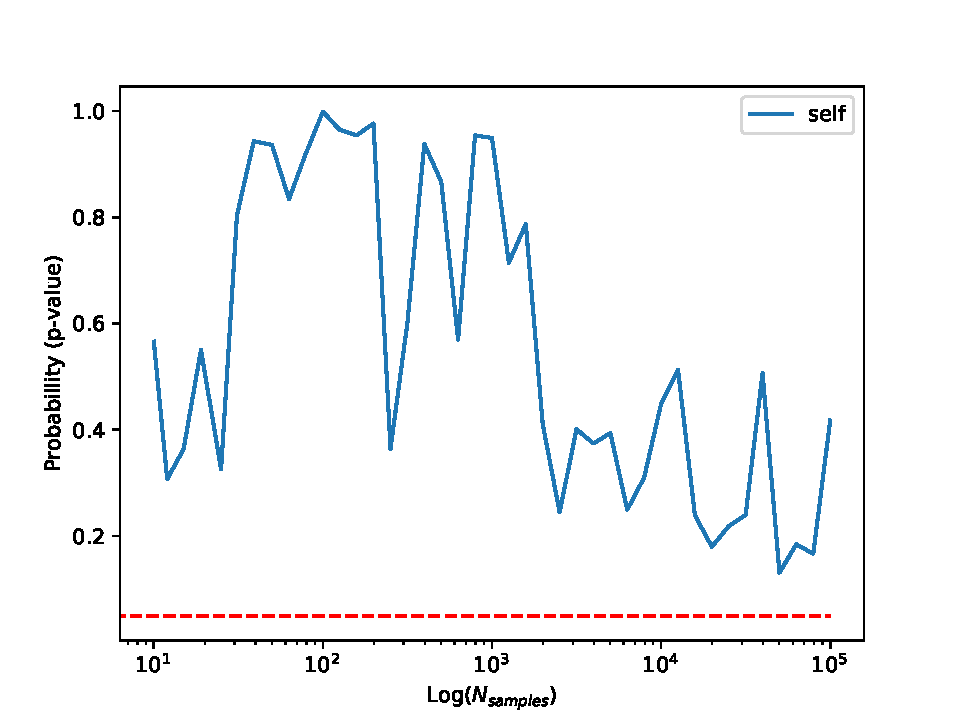
\includegraphics[width=12cm, height=7.5cm]{./Plots/1_plot_kuiper_test_self.pdf}
\caption{The P-value produced by the kuiper test against the number of samples on which the kuiper-test is performed for the self written RNG. The red line indicates the line of $ p = 0.05$. A point \textbf{below} there  line would suggests that there is enough statistical evidence to reject the (null) hypothesis that the data is normal distributed. The plot shows that the RNG always passes kuiper test. IT can however be seen that the value of the statistic stays lower for a significant amount of samples ($ N_{samples} > 10^4$). This might indicate that there is flaw in the random number generator.}
\end{figure}

\begin{figure}[!hb]
\centering
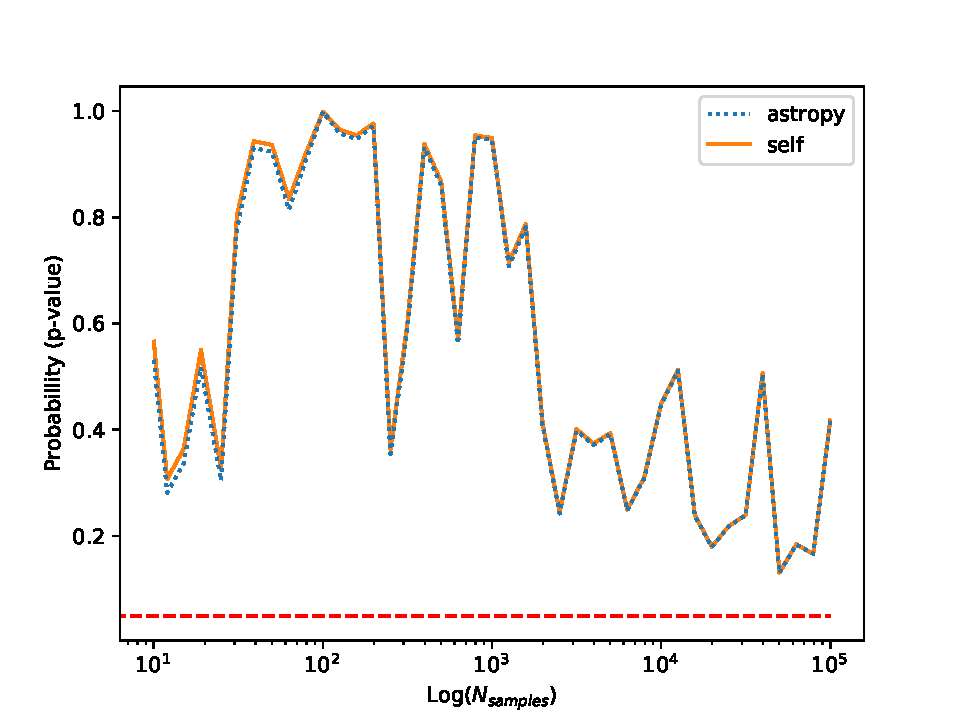
\includegraphics[width=12cm, height=7.5cm]{./Plots/1_plot_kuiper_test_self_astropy.pdf}
\caption{The P-value produced by the kuiper test against the number of samples on which the kuiper-test is performed for the self written RNG. The red line indicates the line of $ p = 0.05$. A point \textbf{below} there  line would suggests that there is enough statistical evidence to reject the (null) hypothesis that the data is normal distributed. The plot shows that the self written implementation deviates from the astropy implementation at the start, similar to what happend in the KS-test.   }
\end{figure}

\end{quote}



\end{quote}

\newpage

%\textbf{Code - output } 
%\begin{quote}
% The code that produces the output.
%\lstinputlisting{./code/assigment1_a.py}
%\end{quote}

%\textbf{Code - helper } 
%\begin{quote}
%The code for the Poisson distribution and the factorial function.  
%\lstinputlisting[firstline=2,lastline=46]{./code/mathlib/utils.py}
%\end{quote}


%\textbf{Output}
%\begin{quote}
%The output produced by \textsf{/code/assigment1\_ a.py} 
%\lstinputlisting{./output/assigment1_a_out.txt}
%\end{quote}
\newpage











